\documentclass[12pt,a4paper]{article}

% Paquetes básicos
\usepackage[utf8]{inputenc}
\usepackage[spanish]{babel}
\usepackage{graphicx}
\usepackage{grffile}
\usepackage{geometry}
\usepackage{hyperref}
\usepackage{float}
\usepackage{titlesec}
\usepackage{caption}
\usepackage{fancyhdr}
\usepackage{xcolor}

% Configuración de márgenes
\geometry{left=2.5cm, right=2.5cm, top=3cm, bottom=2.5cm}
\setlength{\headheight}{15pt} % Solución a la advertencia de fancyhdr

% Configuración de encabezados y pies de página
\pagestyle{fancy}
\fancyhf{}
\lhead{\textcolor{gray}{Portafolio de Evidencias}}
\rhead{\textcolor{gray}{Miguel Angel Peralta Cano}}
\cfoot{\thepage}
\renewcommand{\headrulewidth}{0.4pt}

% Configuración de enlaces
\hypersetup{
    colorlinks=true,
    linkcolor=black,
    filecolor=blue,      
    urlcolor=blue,
    pdftitle={Portafolio de Evidencias - Análisis y Gestión de Logs},
}

\begin{document}

% -----------------------------------------------------------
% 1. PORTADA TIPO ARTÍCULO Y RESUMEN
% -----------------------------------------------------------
\thispagestyle{empty}

\begin{center}
    {\Large \textbf{Fundación Politécnico Minuto de Dios}}\par
\end{center}

\vspace{1.5cm}

\begin{center}
    {\LARGE \textcolor{blue!70!black}{\textbf{PRÁCTICA SOBRE ANÁLISIS Y}}}\\[0.4cm]
    {\LARGE \textcolor{blue!70!black}{\textbf{GESTIÓN DE LOGS E INCIDENTES}}}\\[0.4cm]
    {\LARGE \textcolor{blue!70!black}{\textbf{DE SEGURIDAD}}}\par
\end{center}

\vspace{0.8cm}
\noindent\rule{\textwidth}{0.8pt}
\vspace{0.8cm}

\begin{center}
    {\large \textbf{Materia:} Monitoreo de la Seguridad Informática}\\[0.6cm]
    {\large \textbf{Estudiante:} Miguel Angel Peralta Cano}\\[0.6cm]
    {\large \textbf{Docente:} José Luis Rodríguez Cortés}\\[0.8cm]
    {\large 9 de junio de 2026}\par
\end{center}

\vspace{1.2cm}

\begin{center}
    \textbf{Resumen}
\end{center}
\noindent {\small El presente documento constituye un portafolio de evidencias técnico sobre la conceptualización, monitoreo y respuesta a incidentes utilizando registros del sistema (logs). Se aborda la problemática de la seguridad de la información desde una perspectiva eminentemente práctica, documentando la instalación y configuración de la estación de trabajo CyberOps. Mediante el uso de herramientas de línea de comandos en Linux (tales como \texttt{cat}, \texttt{tail}, y \texttt{journalctl}), se auditan eventos del sistema operativo y de red, diagnosticando y rastreando anomalías. Finalmente, se aplica la teoría a un escenario simulado de infección por gusano informático y ataque de Denegación de Servicio (DDoS), estableciendo un protocolo estructurado de respuesta a incidentes apoyado en herramientas de ciberseguridad, basado en las fases de Preparación, Detección, Contención, Erradicación y Recuperación.}\par

\vspace{0.8cm}
\noindent\rule{\textwidth}{0.4pt}

\newpage


% -----------------------------------------------------------
% 2. TABLA DE CONTENIDO
% -----------------------------------------------------------
\renewcommand*\contentsname{Índice}
\tableofcontents
\newpage

% -----------------------------------------------------------
% 3. INTRODUCCIÓN
% -----------------------------------------------------------
\section{Introducción}

En el presente portafolio se recopilan todas las actividades y evidencias operativas desarrolladas durante la práctica de análisis de logs y gestión de incidentes en el entorno controlado de la máquina virtual CyberOps.

\textbf{¿Cuál es el propósito del portafolio?}\\
El propósito fundamental de este documento es registrar, organizar y justificar de manera técnica el paso a paso de la práctica de laboratorio. Sirve como un expediente demostrativo de la asimilación de habilidades prácticas: la ejecución precisa de comandos de Linux para la lectura forense de registros, la correlación de eventos críticos y la arquitectura de soluciones tácticas ante incidentes de ciberseguridad. Representa el puente necesario entre la teoría de los marcos de control y la trinchera técnica operativa.

\textbf{¿Cuál es su importancia?}\\
Su importancia radica en la capacidad de forzar una reflexión analítica sobre la instrumentación utilizada. En seguridad informática, operar en la línea de comandos sin comprender el subtexto es ineficaz; es indispensable argumentar \textit{por qué} una herramienta específica (como \texttt{less} vs \texttt{more}) ahorra minutos vitales durante un ataque. Los registros (logs) son la materia prima indiscutible de cualquier autopsia digital; comprenderlos y estructurar un plan de respuesta en fases asegura que la organización no dependa de la improvisación frente a una crisis.

\subsection*{Justificación del Formato de Documentación}

Este informe técnico ha sido maquetado y compilado utilizando el sistema de composición de textos \LaTeX. La elección de esta herramienta se fundamenta en su estatus como estándar de facto para la redacción de documentos científicos e ingenieriles. \LaTeX{} garantiza una presentación estructurada, modular y altamente profesional, con un manejo matemático del espaciado y una renderización exacta de los bloques de código y salidas de terminal (CLI). Estas características aseguran que los reportes de auditoría y respuesta a incidentes sean pulcros, legibles y cumplan con los estándares visuales de la industria corporativa.

% -----------------------------------------------------------
% 4. CONTENIDO (DESARROLLO DE LA PRÁCTICA)
% -----------------------------------------------------------
\section{Desarrollo de la Actividad Práctica}

\subsection{Práctica 1: Instalación de la máquina virtual de la estación de trabajo CyberOps}

Para iniciar el entorno de simulación, se procedió con la instalación de Oracle VirtualBox y la importación de la imagen (\textit{appliance}) en formato OVA de la máquina CyberOps Workstation. Durante este proceso, se impuso la reinicialización de la dirección MAC de la interfaz de red, una práctica vital para evitar colisiones de enrutamiento y suplantaciones de identidad (ARP Spoofing) en laboratorios de red.

Tras el arranque del sistema invitado, se inició sesión utilizando las credenciales asignadas (\textit{analista / cyberops}). A partir de aquí, se desarrolló el Paso 3 de la guía, familiarizándose con el entorno de la máquina virtual:

\subsubsection*{Paso 3: Familiarícese con la máquina virtual}

\textbf{A. Enumere las aplicaciones en el menú CyberOps.}\\
\textbf{Rta:} Dentro del menú especializado de \textbf{CyberOps}, se identificaron las siguientes aplicaciones y accesos directos principales:
\begin{itemize}
    \item Mostrar el escritorio (\textit{Show Desktop}).
    \item Aplicación terminal (\textit{Terminal Emulator}).
    \item Aplicación de administrador de archivos (\textit{File Manager}).
    \item Aplicación de navegador web (\textit{Web Browser - Firefox}).
    \item Herramienta de búsqueda de archivos (\textit{Search Tool}).
    \item Directorio de inicio del usuario actual (\textit{Home Directory}).
\end{itemize}

\begin{figure}[H]
    \centering
    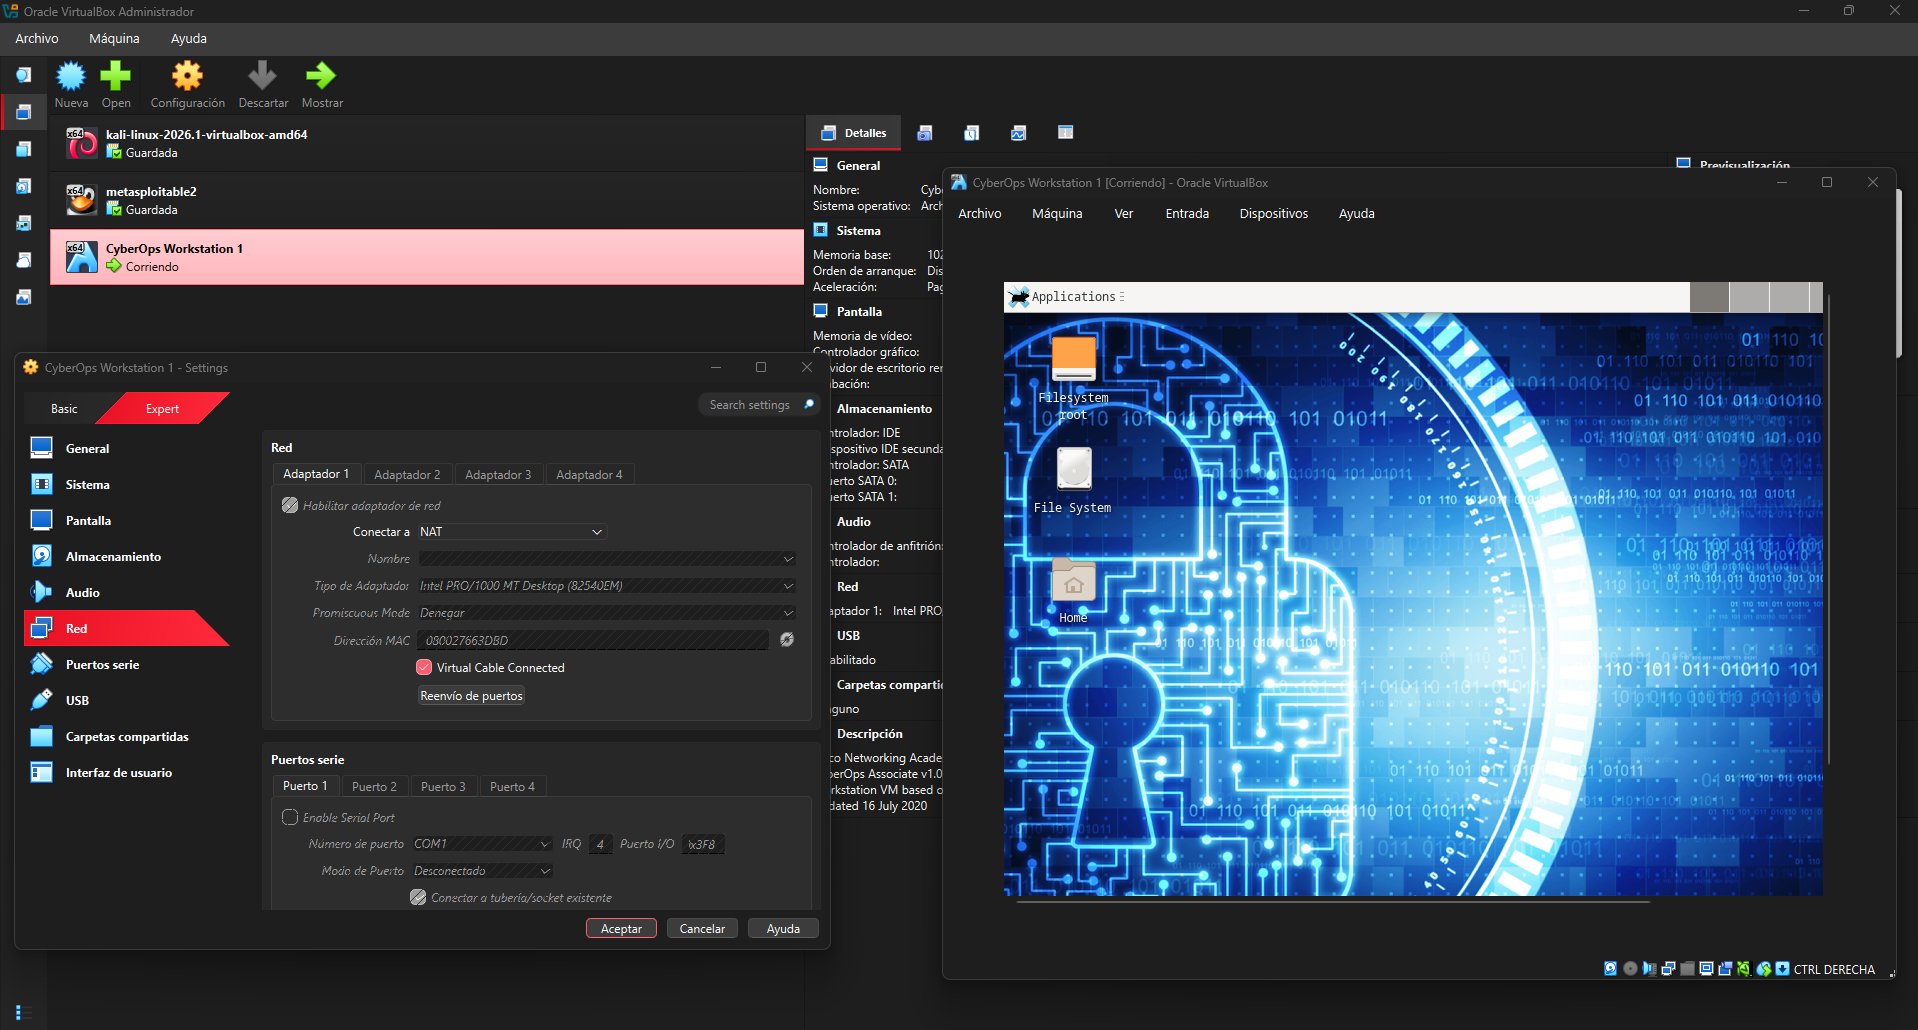
\includegraphics[width=0.9\textwidth]{Imagenes_de_evidencia/Inicio_maquina_CyberOps.png}
    \caption{Pantalla de inicio e interfaz de la máquina CyberOps Workstation, evidenciando el entorno aislado.}
\end{figure}

\textbf{B. Abra la aplicación Terminal Emulator. Escriba ip address en el indicador para determinar la dirección IP de su máquina virtual. ¿Cuáles son las direcciones IP asignadas a su máquina virtual?}\\
\textbf{Rta:} Al ejecutar el comando \texttt{ip address}, se identifican dos interfaces de red. La interfaz de bucle local (\texttt{lo}) tiene asignada la dirección \texttt{127.0.0.1}. Por otro lado, la interfaz de red principal (\texttt{enp0s3}), que nos provee conectividad externa, tiene asignada dinámicamente la dirección IPv4 \textbf{10.0.2.15/24}.

\begin{figure}[H]
    \centering
    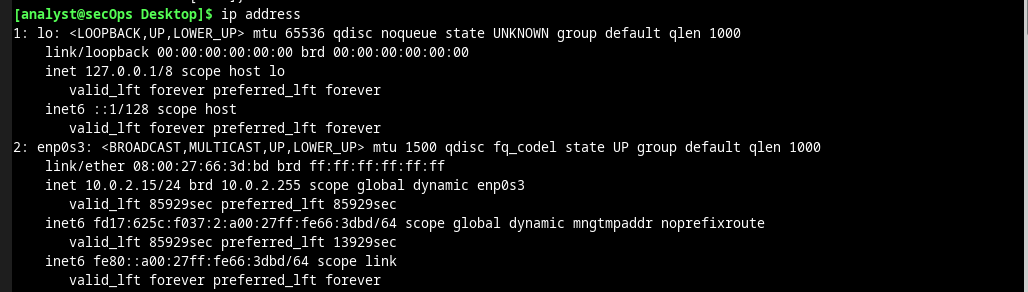
\includegraphics[width=0.8\textwidth]{Imagenes_de_evidencia/ip_address.png}
    \caption{Verificación de la pila TCP/IP y dirección IP asignada a la interfaz de la máquina virtual.}
\end{figure}

\textbf{C. Busque e inicie la aplicación del navegador web. ¿Puede navegar hasta su motor de búsqueda favorito?}\\
\textbf{Rta:} Sí, al ejecutar el navegador web integrado (Firefox) se logra navegar exitosamente hacia motores de búsqueda externos (como Google). Esto confirma que tanto la traducción de direcciones de red (NAT) como la resolución de nombres de dominio (DNS) a través del equipo anfitrión operan sin inconvenientes.

\subsubsection*{Paso 4: Apague las máquinas virtuales}

\textbf{Reflexión: ¿Cuáles son las ventajas y desventajas de usar una máquina virtual?}
\begin{itemize}
    \item \textbf{Ventajas y Casos de Uso Reales:} La virtualización otorga aislamiento criptográfico y de memoria (\textit{Sandboxing}). En la vida real, los analistas de malware (Malware Analysts) ejecutan virus destructivos (como Ransomware) exclusivamente dentro de máquinas virtuales. Si el sistema colapsa, no infecta el equipo anfitrión (\textit{Host}) y la máquina puede ser restaurada a su estado original en segundos mediante "Snapshots" (instantáneas). Además, se utilizan para desplegar \textit{Honeypots} (sistemas trampa) de bajo costo para despistar atacantes.
    \item \textbf{Desventajas y Consideraciones Técnicas:} La principal limitante es el sobrecosto de recursos computacionales (\textit{Overhead}). El anfitrión debe dividir su memoria RAM, núcleos de CPU y almacenamiento físico. En entornos empresariales de alta densidad, una mala asignación de recursos (\textit{Resource Contention}) puede generar cuellos de botella (I/O Bottlenecks), provocando lentitud masiva tanto en el hipervisor como en los sistemas invitados.
\end{itemize}

\subsection{Práctica 2: Lectura de registros (Logs) del servidor}

Los archivos de registro (Logs) son el sistema nervioso central del monitoreo informático. Representan secuencias inmutables de eventos. En esta práctica, se exploró el archivo \texttt{logstash-tutorial.log} utilizando herramientas fundamentales de UNIX/Linux, evaluando la idoneidad de cada una para distintos escenarios de ciberseguridad.

\subsubsection{Inspección Básica y Filtrado (cat, more, less, tail)}

Se inició utilizando el comando de concatenación \texttt{cat}. Al invocarlo, el motor del sistema operativo volcó inmediatamente todo el búfer de texto en la pantalla estándar (\textit{stdout}).

\begin{figure}[H]
    \centering
    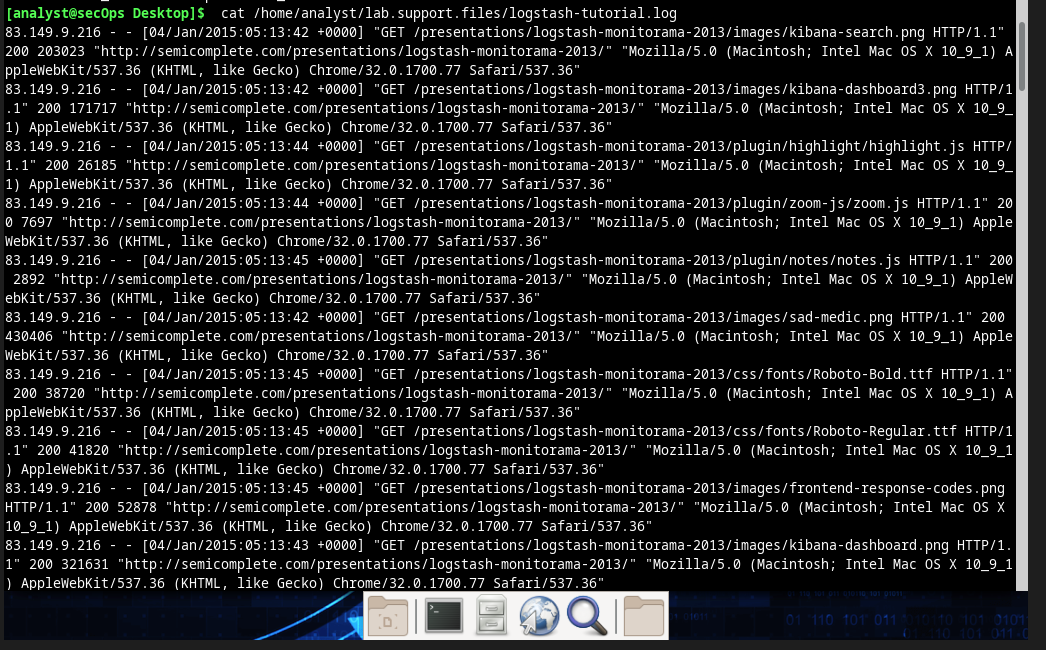
\includegraphics[width=0.8\textwidth]{Imagenes_de_evidencia/cat__home_analyst_lab.support.files_logstash-tutorial.log.png}
    \caption{Volcado ininterrumpido del archivo mediante cat.}
\end{figure}

\textbf{Aplicación Real:} \texttt{cat} es pésimo para logs grandes porque inunda la terminal. Sin embargo, en la vida real, se utiliza combinado con redirecciones (\texttt{>}) o concatenado con el comando \texttt{grep} para extraer rápidamente información, por ejemplo: \texttt{cat /var/log/auth.log | grep "Failed password"} para cazar intentos de fuerza bruta.

Posteriormente, se introdujo el paginador \texttt{more}. Esto frenó el flujo de texto, permitiendo leer el registro bloque a bloque.\\
\textbf{¿Cuál es el inconveniente de usar more?} El obstáculo arquitectónico de \texttt{more} es su unidireccionalidad. Solo permite avanzar (Scroll Down). En un análisis forense, si el ingeniero detecta una IP maliciosa y accidentalmente presiona la barra espaciadora, no puede retroceder para revisar el contexto previo del ataque sin tener que cerrar la herramienta y volver a empezar.

\begin{figure}[H]
    \centering
    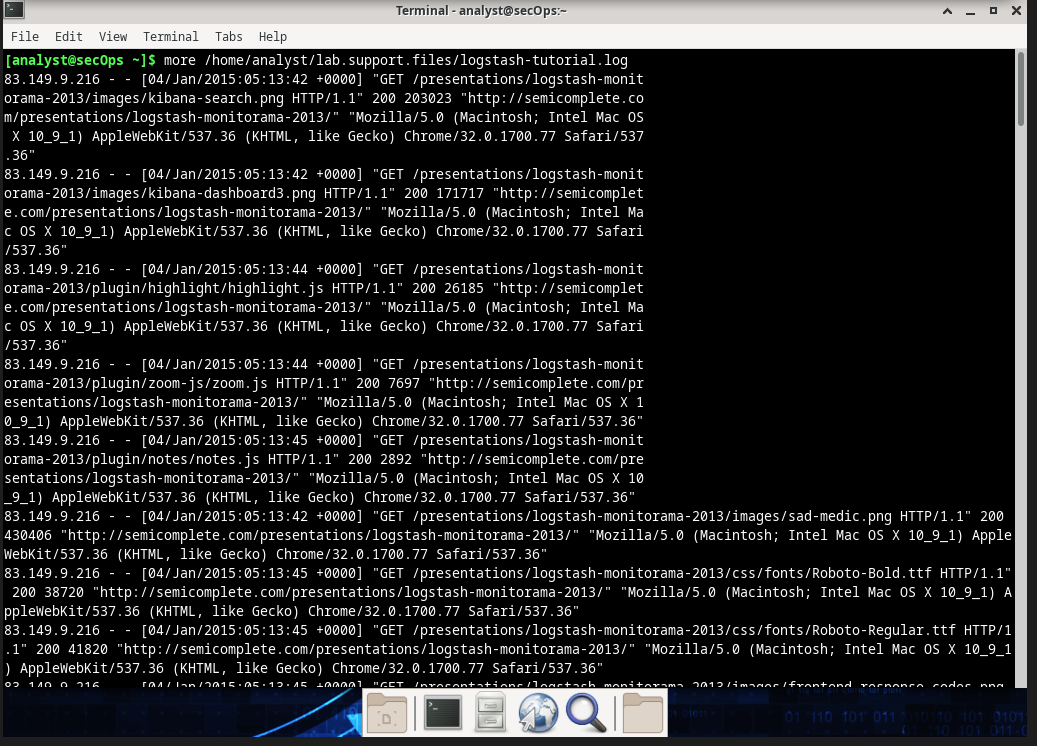
\includegraphics[width=0.8\textwidth]{Imagenes_de_evidencia/more__home_analyst_lab.support.files_logstash-tutorial.log.png}
    \caption{Visualización paginada y unidireccional con more.}
\end{figure}

Para mitigar esta ineficiencia, se desplegó \texttt{less}. Esta herramienta no carga el archivo completo en la memoria RAM, lo que la hace ultrarrápida incluso con logs de varios Gigabytes.

\begin{figure}[H]
    \centering
    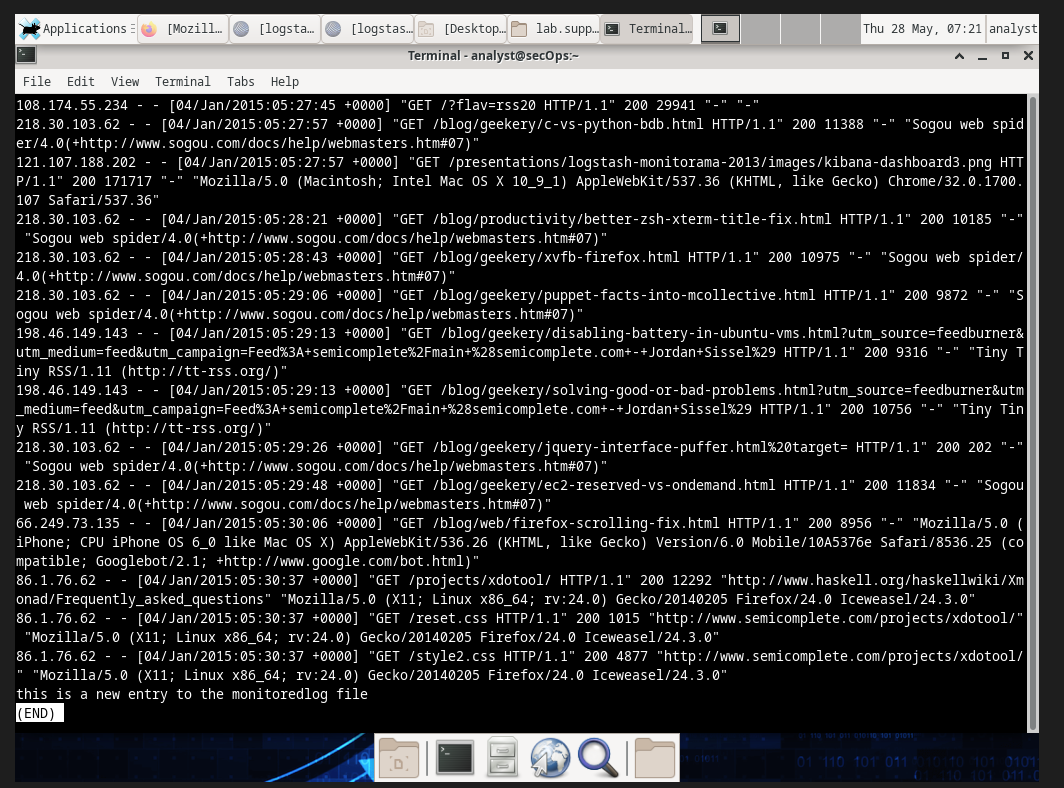
\includegraphics[width=0.8\textwidth]{Imagenes_de_evidencia/less__home_analyst_lab.support.files_logstash-tutorial.log.png}
    \caption{Navegación dinámica y bidireccional usando less.}
\end{figure}

\textbf{Aplicación Real:} \texttt{less} permite búsquedas con expresiones regulares interactivas escribiendo \texttt{/} seguido de una palabra (ej. \texttt{/ERROR}). Es la herramienta preferida en los NOC (Network Operations Centers) para buscar transacciones perdidas sin colgar el servidor.

Finalmente, el comando \texttt{tail} resolvió la necesidad de ver únicamente las transacciones más recientes (por defecto, las últimas 10 líneas).

\begin{figure}[H]
    \centering
    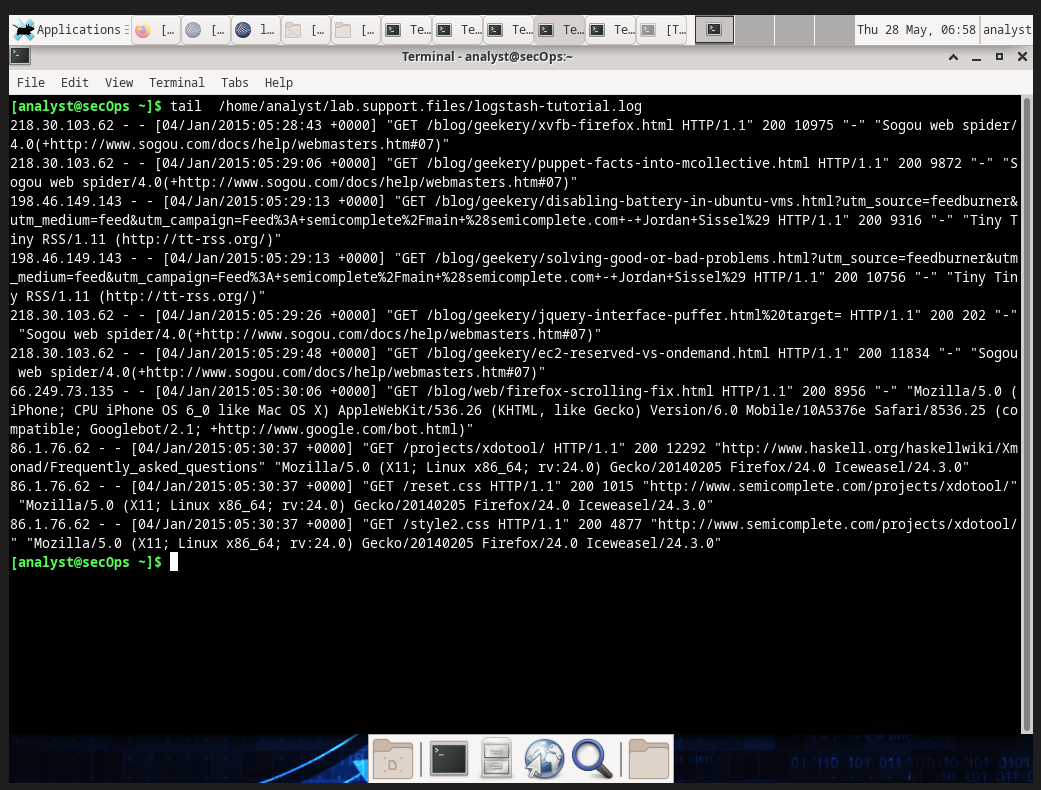
\includegraphics[width=0.8\textwidth]{Imagenes_de_evidencia/tail__home_analyst_lab.support.files_logstash-tutorial.log.png}
    \caption{Extracción de las últimas transacciones registradas usando tail.}
\end{figure}

\subsubsection{Monitorización Activa: Trazabilidad en Tiempo Real}

Para escenarios críticos, un registro estático es insuficiente. Se dividió la pantalla en dos terminales: en la primera se ejecutó el comando de seguimiento \texttt{tail -f}, y en la segunda se inyectó una cadena de texto manual mediante \texttt{echo} redirigida al archivo monitoreado.

\begin{figure}[H]
    \centering
    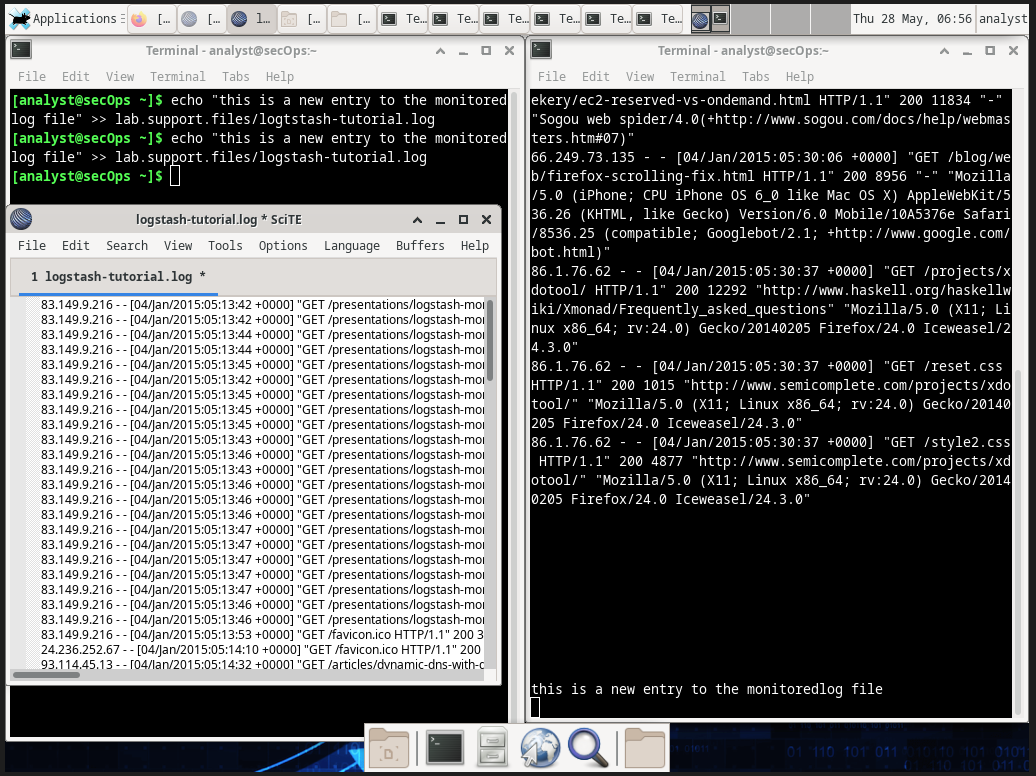
\includegraphics[width=0.9\textwidth]{Imagenes_de_evidencia/Seguimiento_activo_de_los_registros_-_sudo_tail_-f_y_echo_.png}
    \caption{Prueba de concepto de monitorización en vivo capturando escrituras en tiempo real.}
\end{figure}

\textbf{¿Qué es diferente en la salida de tail y tail -f? Explique.}\\
El comando \texttt{tail} tradicional es \textit{post-mortem}: lee el estado del archivo en ese milisegundo y cierra el proceso. Por el contrario, el modificador \texttt{-f} (follow) mantiene el descriptor del archivo (File Descriptor) abierto en la memoria RAM.
En un entorno real de producción corporativa, \texttt{tail -f /var/log/nginx/access.log} le permite al administrador observar un ataque de inyección SQL (SQLi) o un escaneo de vulnerabilidades web en el instante exacto en que los paquetes HTTP están golpeando el servidor web, habilitando una respuesta instantánea.

\subsubsection{Syslog y Privilegios del Sistema}

Se exploró la ubicación estándar de registros en Linux: \texttt{/var/log}. Al intentar acceder a los registros centrales (\texttt{syslog.1}), el sistema denegó la lectura, requiriendo el uso de \texttt{sudo} (Super User DO).

\begin{figure}[H]
    \centering
    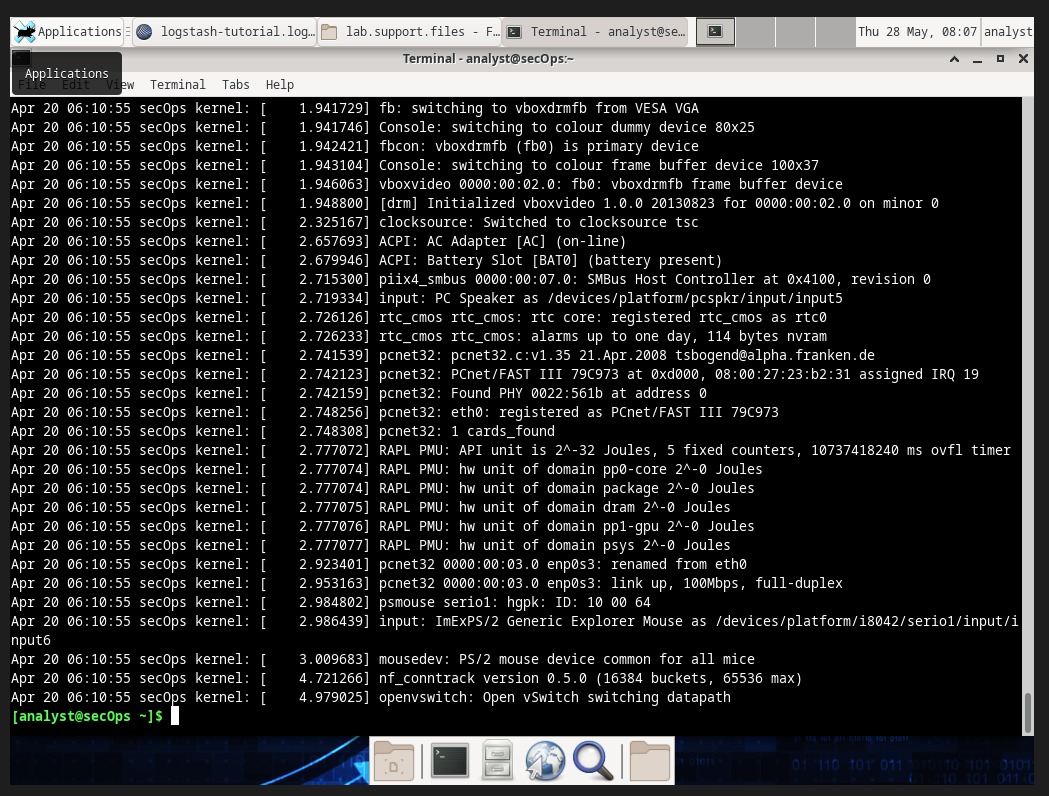
\includegraphics[width=0.8\textwidth]{Imagenes_de_evidencia/sudo_cat__var_log_syslog.1.png}
    \caption{Auditoría de registros del sistema mediante escalada de privilegios.}
\end{figure}

\textbf{¿Por qué el comando cat tuvo que ejecutarse como root?}\\
El principio de Menor Privilegio (PoLP). El archivo \texttt{syslog} documenta eventos del Kernel, fallos de montaje de hardware, y más importante, rastros de autenticación (quién entró, a qué hora, qué comandos se ejecutaron). Si un atacante lograra vulnerar un usuario estándar no privilegiado, la restricción de lectura de estos logs impide que realice un reconocimiento interno (Reconnaissance) o que borre sus huellas.

La infraestructura utiliza rotación de logs (Log Rotation) para prevenir que los archivos de texto colapsen el almacenamiento físico (\textit{Out of Space}). A continuación se auditaron los archivos históricos rotados \texttt{syslog.2}, \texttt{syslog.3} y \texttt{syslog.4}:

\begin{figure}[H]
    \centering
    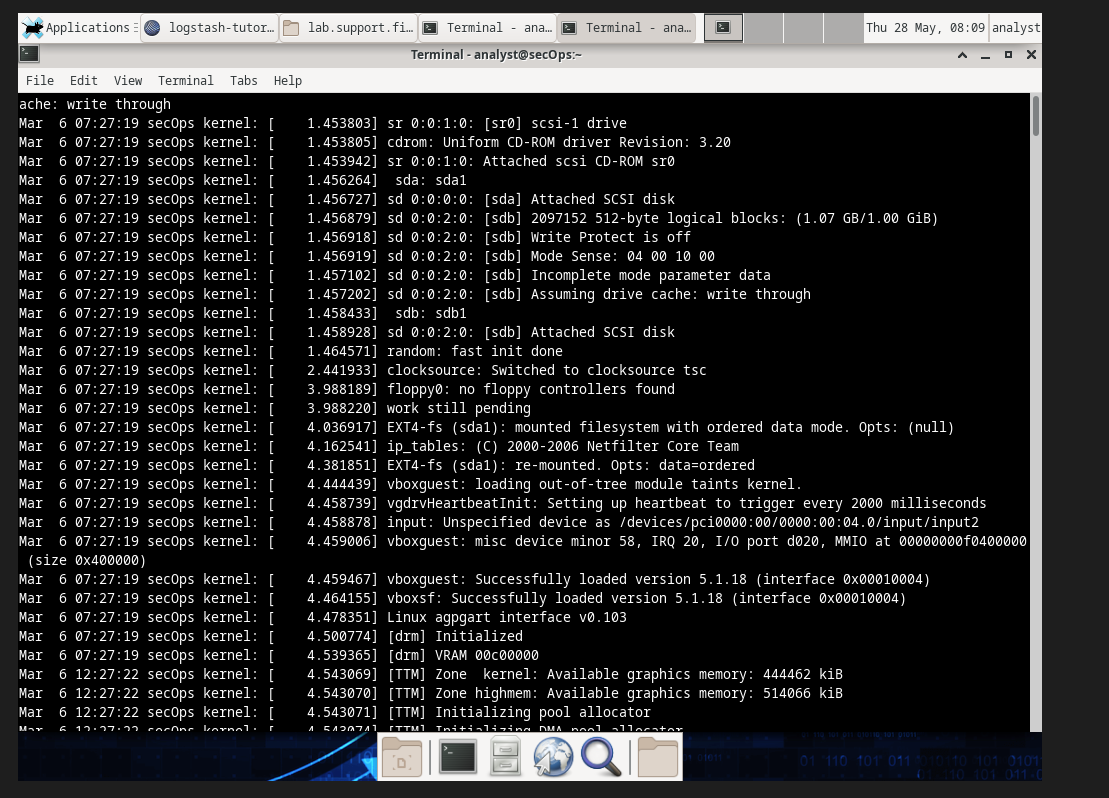
\includegraphics[width=0.45\textwidth]{Imagenes_de_evidencia/sudo_cat__var_log_syslog.2.png}
    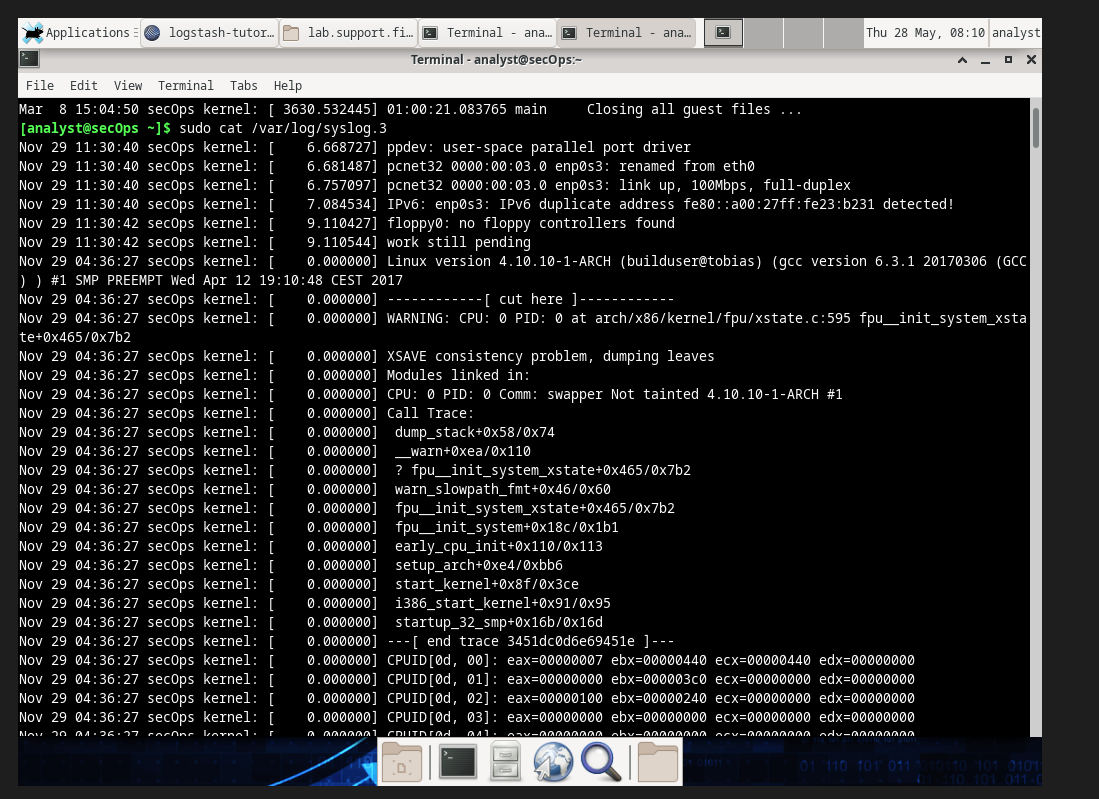
\includegraphics[width=0.45\textwidth]{Imagenes_de_evidencia/sudo_cat__var_log_syslog.3.png}
    \\[0.5cm]
    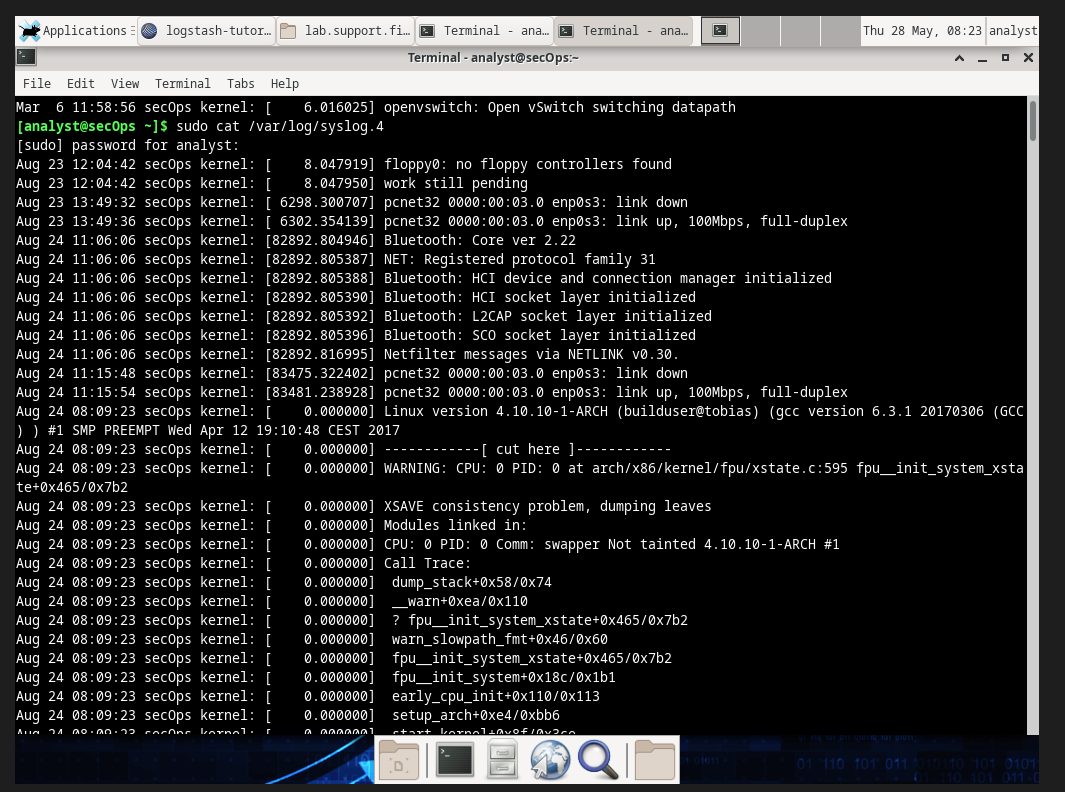
\includegraphics[width=0.45\textwidth]{Imagenes_de_evidencia/sudo_cat__var_log_syslog.4.png}
    \caption{Examen de archivos rotados y empaquetados por el demonio logrotate.}
\end{figure}

\textbf{¿Por qué es tan importante mantener la fecha y la hora de los computadores correctamente sincronizadas?}\\
El impacto de un reloj desfasado es catastrófico para la correlación de eventos. En la respuesta a incidentes, los ataques suelen ser cadenas complejas (ej. Infección a las 10:00:01, Escalamiento a las 10:00:03, Exfiltración a las 10:00:10). Si el servidor Web tiene una hora distinta a la del Servidor de Base de Datos, el SIEM (Gestor de Seguridad) será incapaz de trazar la ruta de ataque linealmente. El uso del protocolo NTP (Network Time Protocol) es un requisito normativo ineludible para garantizar la validez legal de las pruebas informáticas.

\subsubsection{La Evolución: Archivos de registro y Journalctl}

Los entornos basados en Systemd abandonan los logs en texto plano en favor del demonio \texttt{journald}. Este sistema indexa los registros en una base de datos binaria altamente estructurada.

\begin{figure}[H]
    \centering
    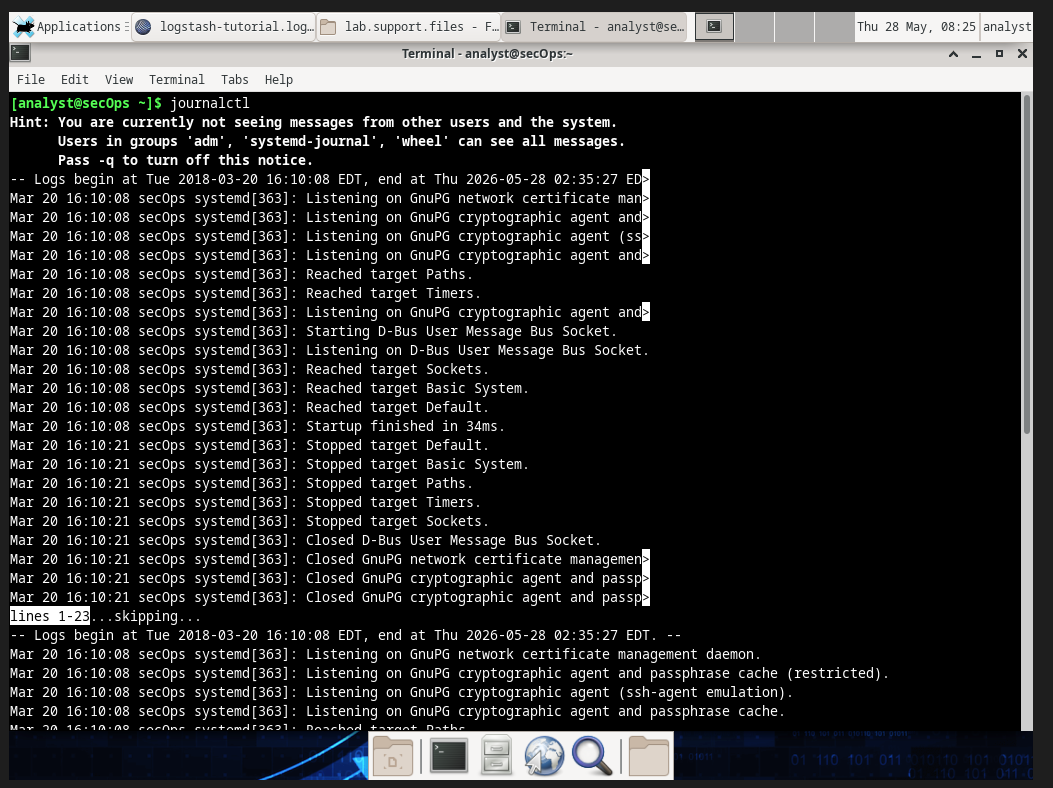
\includegraphics[width=0.8\textwidth]{Imagenes_de_evidencia/journalctl.png}
    \caption{Vista estandarizada de la base de datos de logs mediante journalctl.}
\end{figure}

La potencia de \texttt{journalctl} reside en sus capacidades de consulta sintáctica (\textit{Querying}). Se experimentó con múltiples parámetros de filtrado forense:

\begin{itemize}
    \item \texttt{journalctl --utc}: Normaliza todas las marcas de tiempo al meridiano de Greenwich (UTC). Crítico para empresas transnacionales.
    \item \texttt{journalctl -b}: (\textit{Boot}) Filtra agresivamente la base de datos para mostrar única y exclusivamente los eventos que ocurrieron desde el último reinicio del servidor, descartando meses de datos irrelevantes.
    \item \texttt{journalctl -k}: (\textit{Dmesg/Kernel}) Suprime los mensajes de aplicaciones (Capa 7) y aísla los mensajes del anillo cero (Ring 0) del sistema operativo, vital para diagnosticar fallos de hardware o pánicos del núcleo (\textit{Kernel Panics}).
    \item \texttt{journalctl -u nginx.service}: Aísla los registros pertenecientes exclusivamente a una unidad de servicio (en este caso el servidor web Nginx).
\end{itemize}

\begin{figure}[H]
    \centering
    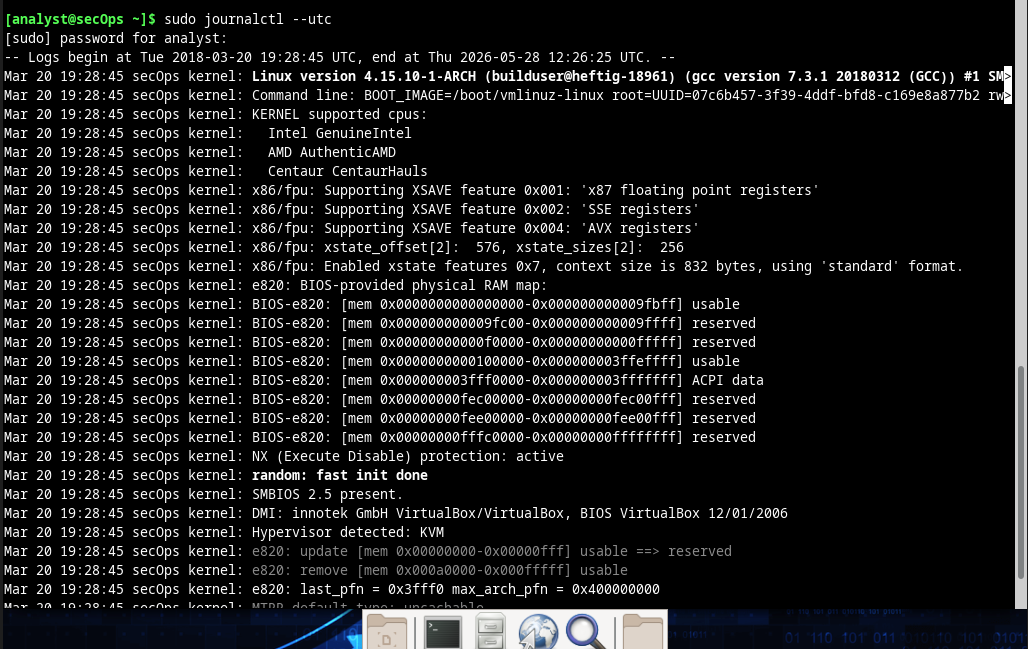
\includegraphics[width=0.45\textwidth]{Imagenes_de_evidencia/sudo_journalctl_--utc.png}
    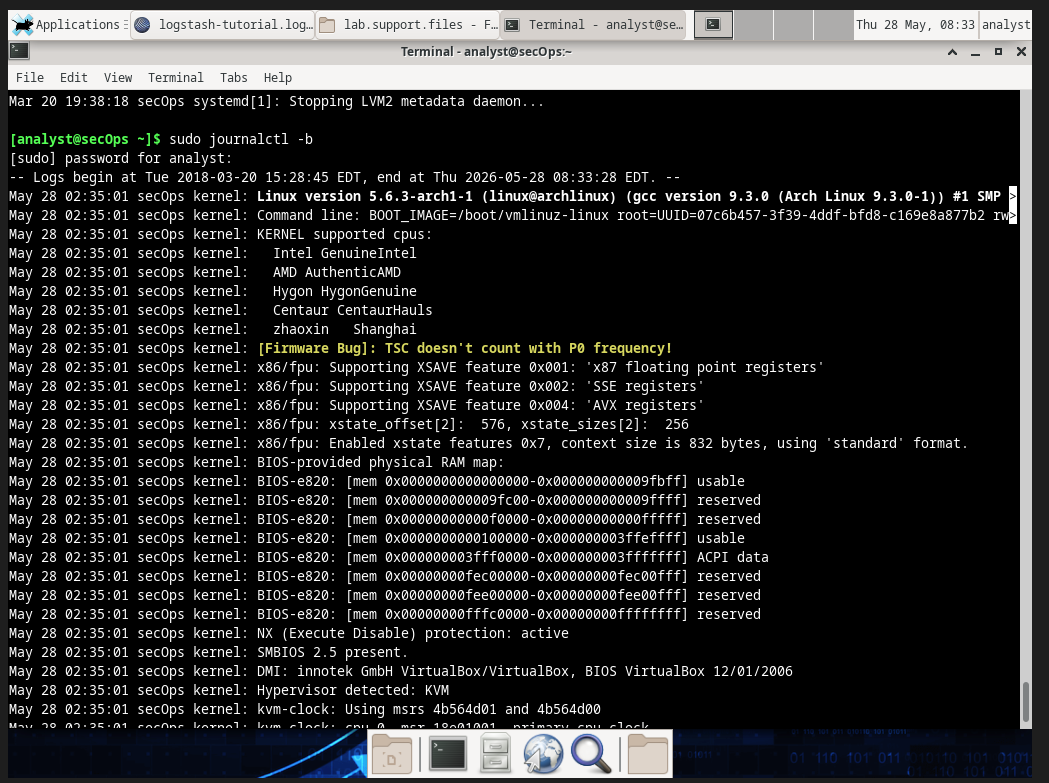
\includegraphics[width=0.45\textwidth]{Imagenes_de_evidencia/sudo_journalctl_–b.png}
    
    \vspace{0.5cm}
    
    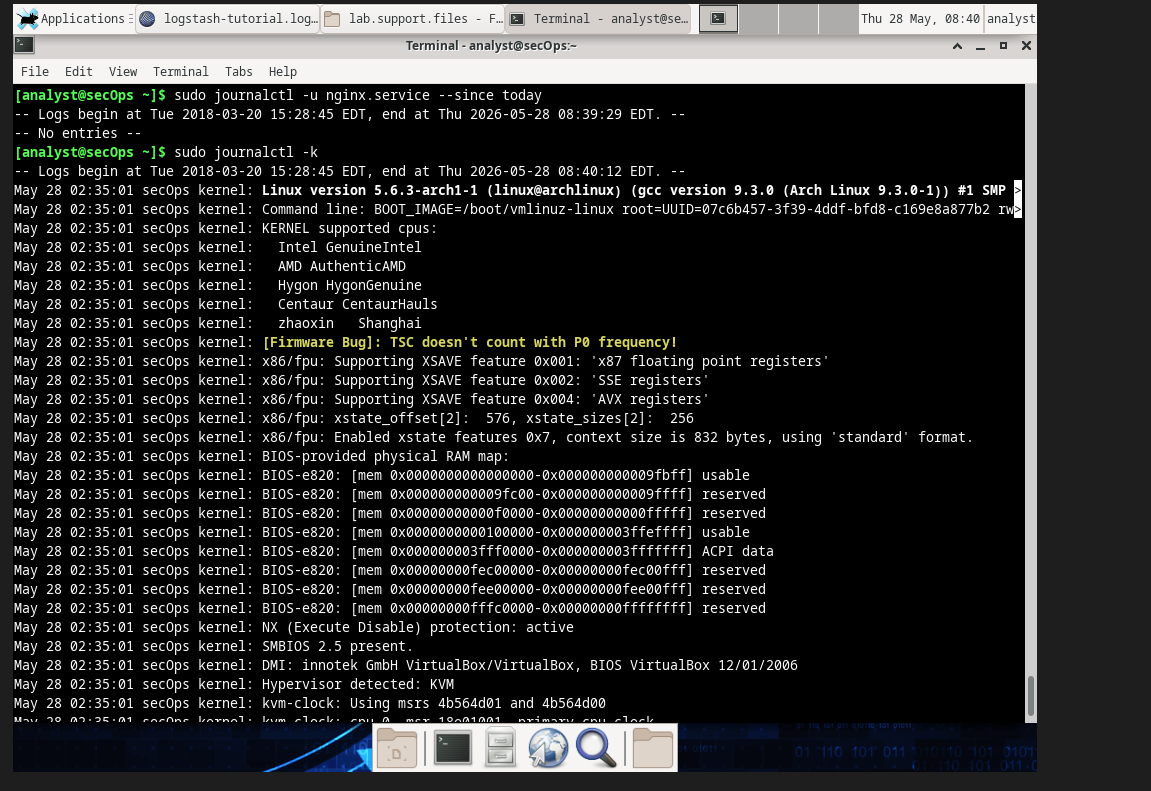
\includegraphics[width=0.45\textwidth]{Imagenes_de_evidencia/sudo_journalctl_–k.png}
    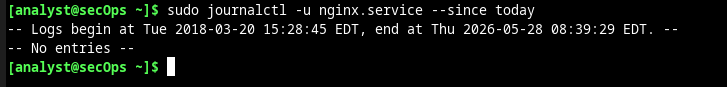
\includegraphics[width=0.45\textwidth]{Imagenes_de_evidencia/sudo_journalctl_-u_nginx.service_--since_today.png}
    \caption{Aplicación de la doctrina de filtrado técnico con modificadores journalctl.}
\end{figure}

\textbf{Reflexión Técnica: Compare Syslog y Journald. ¿Cuáles son las ventajas y desventajas de cada uno?}
\begin{itemize}
    \item \textbf{Syslog (El Estándar Clásico):} Su ventaja definitiva es la ubicuidad y la simplicidad. Al ser archivos de texto en texto claro (Plaintext), pueden ser procesados mediante potentes herramientas tradicionales de UNIX (\texttt{grep}, \texttt{awk}, \texttt{sed}) y exportados a cualquier SIEM sin adaptadores complejos. Su desventaja recae en la falta de metadatos integrados; la manipulación o parseo de logs requiere el uso de expresiones regulares densas y propensas a errores.
    \item \textbf{Journald (El Enfoque Moderno):} Su inmensa ventaja es la integridad y el filtrado metadato. Al ser binario, permite consultar logs por PID (Process ID), UID (Usuario) o UUID de máquina instantáneamente. Incluso soporta salida nativa en formato JSON (\texttt{-o json}), ideal para ingestas en APIs modernas. Su desventaja es la opacidad: si el binario del journal se corrompe, el administrador no puede recuperar los logs abriéndolos con un bloc de notas simple; se requiere obligatoriamente una herramienta en funcionamiento compatible con la firma binaria de Systemd.
\end{itemize}

\subsection{Práctica 3: Manejo de Incidentes (Estudio de Caso Analítico)}

El escenario plantea una crisis sistémica: Una empresa financiera de 100 empleados es víctima de la propagación incontrolada de un gusano informático de tipo Día Cero (\textit{Zero-Day}) distribuido vía dispositivos de almacenamiento USB y medios compartidos de Windows (Protocolo SMB/CIFS). El malware incluye un \textit{payload} (carga útil) que transforma las estaciones de trabajo en agentes "Zombis" dentro de una Botnet para ejecutar ataques de Denegación de Servicio Distribuido (DDoS). Los motores antivirus clásicos basados en firmas (\textit{Signature-based}) fueron ineficaces durante horas.

Para abordar este incidente, se deben responder las preguntas estratégicas del modelo de respuesta a incidentes (NIST SP 800-61), estructurando así nuestro plan de acción:

\subsubsection{Fase 1: Preparación}
\begin{itemize}
    \item \textbf{¿La organización consideraría esta actividad como un incidente? Si es así, ¿cuál de las políticas de la organización viola esta actividad?}\\
    Absolutamente. Se clasifica como un Incidente Crítico de Seguridad (Prioridad 1) debido a la interrupción operativa y al riesgo de participación involuntaria en un ciberataque externo (DDoS). Viola frontalmente las "Políticas de Uso Aceptable de Dispositivos Extraíbles (USB)", la "Política de Tráfico de Red Permitido" y la "Política de Seguridad de Endpoint".
    \item \textbf{¿Qué medidas existen para intentar evitar que este tipo de incidente vuelva a ocurrir o limitar su impacto?}\\
    Para prevenir, se debe implementar una Política de Grupo (GPO) a nivel de Active Directory que bloquee el montaje de la clase \texttt{USBSTOR} (memorias USB no autorizadas). Para limitar el impacto, se debe forzar el aislamiento de red (Microsegmentación VLAN) y desplegar plataformas \textit{Endpoint Detection and Response} (EDR, ej. SentinelOne, CrowdStrike) que bloquean malware por comportamiento anómalo, en lugar de depender de firmas de antivirus tradicionales.
\end{itemize}

\subsubsection{Fase 2: Detección y Análisis}
\begin{itemize}
    \item \textbf{¿Qué precursores del incidente, si los hay, podría detectar la organización?}\\
    Un precursor claro habría sido el registro de intentos masivos de conexión fallida a los puertos SMB (TCP 445) desde máquinas internas hacia recursos compartidos (comportamiento típico de un gusano mapeando la red).
    \item \textbf{¿Qué indicadores del incidente podría detectar la organización?}\\
    Los indicadores principales (IoCs) incluyen: lentitud extrema de la red interna (causada por el tráfico lateral del gusano), alertas del Firewall perimetral reportando un inusual volumen de tráfico UDP/TCP saliente coordinado hacia direcciones IP externas desconocidas (el ataque DDoS), y picos de consumo de CPU/RAM al 100\% en las estaciones de los asesores.
    \item \textbf{¿Qué herramientas adicionales podrían ser necesarias para detectar este incidente en particular?}\\
    Es imperativo el uso de un \textbf{SIEM} (Wazuh, Splunk) para centralizar la telemetría, y Sistemas de Detección de Intrusos (\textbf{NIDS} como Snort o Suricata) para analizar los paquetes en tránsito y levantar alertas sobre tráfico malicioso antes de que el antivirus local se percate.
    \item \textbf{¿Cómo priorizaría el equipo el manejo de este incidente?}\\
    El incidente debe catalogarse como \textbf{Severidad Alta/Crítica}. El equipo debe priorizar primero detener el tráfico saliente (DDoS) para evitar daños legales y reputacionales (responsabilidad civil), y en segundo lugar, frenar la propagación lateral interna para salvar los servidores de bases de datos.
\end{itemize}

\subsubsection{Fase 3: Contención, Erradicación y Recuperación}
\begin{itemize}
    \item \textbf{¿Qué estrategia debería tomar la organización para contener el incidente? ¿Por qué esta estrategia es preferible a otras?}\\
    La estrategia de \textbf{Contención Dinámica (Aislamiento Lógico)} es la mejor. A través de la CLI del Switch, se envían los puertos de los equipos infectados a una \textit{VLAN de Cuarentena} (sin enrutamiento a Internet ni a servidores internos). Es preferible a simplemente apagar los equipos porque permite mantener la RAM encendida para análisis forense, pero corta instantáneamente la hemorragia de datos y el ataque DDoS. Adicionalmente, el Firewall debe aplicar reglas de bloqueo forzoso (Drop) hacia la IP destino del ataque.
    \item \textbf{¿Qué herramientas adicionales podrían ser necesarias para responder a este incidente?}\\
    Se requerirá \textbf{Wireshark} o \textbf{tcpdump} (a través de un puerto espejo SPAN en el switch) para capturar el tráfico y aislar la IP origen del "paciente cero".
    \item \textbf{¿Qué personal estaría involucrado?}\\
    Administradores de Red (para aislar VLANs y aplicar reglas de Firewall), Analistas de Seguridad SOC/NOC (para analizar logs y trazar el origen), y personal de Soporte Técnico (\textit{HelpDesk}) para asistir en la recuperación física de las máquinas.
    \item \textbf{¿Qué fuentes de evidencia debería adquirir la organización? ¿Cómo se obtendría y almacenaría?}\\
    Se debe realizar un volcado de la memoria RAM (Memory Dump) de los equipos infectados antes de apagarlos (usando herramientas como FTK Imager), y recolectar los logs centralizados (\texttt{syslog}, Event Viewer) desde el SIEM. Esta evidencia debe almacenarse en un servidor seguro (\textit{Cold Storage}) calculando su Hash (SHA-256) para garantizar la Cadena de Custodia. Debe conservarse el tiempo que dicte la normativa legal local (usualmente entre 1 y 5 años) ante posibles demandas del banco afectado por el DDoS.
\end{itemize}

\subsubsection{Fase 4: Actividad Posterior al Incidente}
\begin{itemize}
    \item \textbf{¿Qué se podría hacer para evitar que ocurran incidentes similares en el futuro?}\\
    Implementar el paradigma de \textbf{Zero Trust} (Confianza Cero), exigiendo autenticación multifactor (MFA) para moverse por la red interna. Modificar radicalmente las Políticas de Recursos Humanos imponiendo sanciones severas por conectar dispositivos personales. Deshabilitar los puertos USB mediante políticas del controlador de dominio (GPO).
    \item \textbf{¿Qué se podría hacer para mejorar la detección de incidentes similares?}\\
    Afinar (Tuning) el Firewall y el SIEM para que apliquen bloqueos automatizados. Si un nodo interno comienza a enviar más de 10,000 paquetes por segundo al exterior, la red debe aislarlo automáticamente sin esperar intervención humana. Reemplazar los antivirus estáticos por plataformas EDR impulsadas por Inteligencia Artificial.
\end{itemize}
\newpage

% -----------------------------------------------------------
% 5. CONCLUSIONES
% -----------------------------------------------------------
\section{Conclusiones}

Tras finalizar esta rigurosa actividad práctica, puedo concluir lo siguiente:

En primera instancia, el manejo fluido de registros en sistemas UNIX/Linux mediante comandos como \texttt{tail -f} y \texttt{journalctl} trasciende el mero conocimiento teórico para convertirse en una competencia técnica crítica. Los entornos gráficos (GUI) colapsan o se vuelven ciegos ante ataques volumétricos; es en la interfaz de texto crudo donde el analista de ciberseguridad ejerce la auditoría real y el aislamiento de la falla. Entender las limitantes de carga en memoria de comandos como \texttt{cat} y \texttt{more} frente a la eficiencia forense de \texttt{less} separa a un usuario básico de un administrador avanzado.

En segunda medida, la gestión de incidentes expuso un axioma fundamental de las telecomunicaciones: la correlación es matemáticamente imposible sin relojes sincronizados (NTP). Ningún SIEM de alta tecnología puede reconstruir la cadena de tiempo de un vector de ataque si las estampas de tiempo (Timestamps) están corrompidas por disparidades geográficas.

Por último, frente al escrutinio del estudio de caso, destaco de manera categórica que la ciberseguridad es tridimensional (Personas, Procesos y Tecnología). La excesiva confianza en la respuesta pasiva del software antivirus fue lo que permitió que la botnet DDoS escalara impunemente. La seguridad contemporánea debe ser predictiva y estratificada. Se requiere la visibilidad granular que ofrecen los analizadores de tráfico (\textit{Snort, Wireshark}) y una férrea disciplina corporativa para bloquear vectores primarios físicos (como los puertos USB vía GPO). Contener, erradicar y recuperar no son simples palabras, sino el resultado de un \textit{Playbook} ensayado, financiado e integrado.

\newpage

% -----------------------------------------------------------
% 6. REFERENCIAS BIBLIOGRÁFICAS
% -----------------------------------------------------------
\renewcommand\refname{Referencias Bibliográficas y Técnicas}
\begin{thebibliography}{99}

\bibitem{gomez}
Gómez, Á. (2015). \textit{Gestión de incidentes de seguridad informática}. RA-MA Editorial. Referenciado para las bases metodológicas de la instrumentación de políticas y procesos de contención.

\bibitem{raya}
Raya, L. y Raya, L. (2015). \textit{Sistemas informáticos}. RA-MA Editorial. Citado para el estudio estructural de componentes de sistemas operativos Linux y su vinculación con procesos y anillos del kernel.

\bibitem{chicano}
Chicano, E. (2015). \textit{Gestión de incidentes de seguridad informática (MF0488\_3)}. IC Editorial. Utilizado como marco referencial para establecer directrices de preparación técnica y auditoría en entornos locales.

\bibitem{nist}
Cichonski, P., Millar, T., Grance, T., y Scarfone, K. (2012). \textit{Computer Security Incident Handling Guide} (NIST Special Publication 800-61 Rev. 2). National Institute of Standards and Technology. Estándar canónico implementado para estructurar de manera oficial el ciclo de vida analítico en el Caso de Estudio 3.

\bibitem{blueteam}
Whitehouse, D. (2014). \textit{Blue Team Handbook: Incident Response Edition: A condensed field guide for the Cyber Security Incident Responder.} Análisis aplicado para sustentar la inyección de herramientas en línea de comandos (\texttt{grep, tcpdump, journalctl}) durante eventos de triaje forense activo.

\end{thebibliography}

\end{document}